\documentclass[tikz]{standalone}
\usetikzlibrary{spy,shapes,shadows,calc,pgfplots.groupplots}
\usepackage{amsmath}
\usepackage{physics} 
\usepackage{pgfplots}
\pgfplotsset{compat=1.3}
\usepackage{amsmath}
\DeclareFontFamily{OT1}{pzc}{}
\DeclareFontShape{OT1}{pzc}{m}{it}{<-> s * [1.10] pzcmi7t}{}
\DeclareMathAlphabet{\mathpzc}{OT1}{pzc}{m}{it}
\newcommand{\ddtn}{\operatorname{dtn}}

\pgfplotsset{
  legend style = {font=\small},
   scaled y ticks=false
}

\begin{document}
\begin{tikzpicture}[scale = 1.0]

\begin{scope}[]
\begin{groupplot}[
    group style={
        %group name=rates,
        group size=2 by 1,
        %xticklabels at=edge bottom,
        horizontal sep=30pt,
        vertical sep=40pt,
   },
   %name = dtnplot,
   height = 6cm,
   width = 8.0cm,
   every axis plot/.append style={thick},
   %axis y line*=left,
   %xmin = 0,
   %xmax = 11000,
   %ymin = -20,
   %ymax = 20,
   %restrict y to domain=-1e2:1e2,
   %label style={at={(axis description cs:0.5,-0.08)},anchor=north},
   %every x tick scale label/.style={at={(xticklabel cs:0.925)},anchor=south west},
   x label style={at={(axis description cs:0.35,0.085)},anchor=east},
   %y tick label style = { xshift=-9.5ex, yshift=0.0ex, anchor=west} , 
   %xlabel= { $\lambda$},
   ]
    \nextgroupplot[ 
    ymode=log,
    xmode=log,
    %xmin=0,xmax=1.6e4,
    %xtick={25, 125, 250, 500, 800, 1000},
    %axis x line*=middle,
    %axis y line=middle, 
    xmin = 4e3,
    xmax = 4e6,
    ymin = 3e-2,
    ymax = 2,
    %width=9cm,
    %restrict y to domain=-4e2:4e2,
    %xtick={0,2e3,4e3,6e3,8e3,10e3,12e3,14e3},
    %ytick = {1,0.75,0.5,0.25},  
    xlabel= {ndof},
    %legend pos = south west,
    %legend pos = north east,
    legend style = { column sep = 6pt, legend columns = 3, legend to name = grouplegend,},
    %legend style = { column sep = 2pt, legend columns = 1, anchor=east, legend to name = grouplegend, },
    x label style={at={(axis description cs:0.65,0.075)},anchor=east},
    title = { $p=1$ }, 
    %y tick label style={xshift={3em}}
	]

    \addplot[red,very thick,mark=*] 
	table[x=ndof,y=rel-L2-err-B] {../data/3D-comp-fitted-stab-ip-p1-q1-mus(3,30)-ks(10,30).dat}; \addlegendentry{ fitted $\mu = (3,30)$  } %  
    \addplot[blue,very thick,mark=triangle]  
	table[x=ndof,y=rel-L2-err-B] {../data/3D-comp-unfitted-stab--p1-q1-mus(3,30)-ks(10,30).dat}; \addlegendentry{ unfitted $\mu = (3,30)$  } %  
    \addplot[gray,dashed,thick] 
   	table[mark=none,x=ndof,y expr ={20*\thisrowno{1}}] {../data/3D-comp-unfitted-stab--p1-q1-mus(3,30)-ks(10,30).dat}; \addlegendentry{ $\mathcal{O}(h)$   } %  
    \addplot[red,very thick,dashed,mark=x] 
   	table[x=ndof,y=rel-L2-err-B] {../data/3D-comp-fitted-stab-ip-p1-q1-mus(3,3)-ks(10,30).dat}; \addlegendentry{ fitted $\mu = (3,3)$ } %  
    \addplot[blue,very thick,dashed,mark=diamond]  
	table[x=ndof,y=rel-L2-err-B] {../data/3D-comp-unfitted-stab--p1-q1-mus(3,3)-ks(10,30).dat}; \addlegendentry{ unfitted $\mu = (3,3)$ } %  
    \addplot[gray,densely dotted,thick] 
   	table[mark=none,x=ndof,y expr ={250*\thisrowno{1}*\thisrowno{1}}] {../data/3D-comp-unfitted-stab--p1-q1-mus(3,30)-ks(10,30).dat}; \addlegendentry{ $\mathcal{O}(h^2)$ } %  
    
   \node (meshu) at (axis cs:1.75e4,9e-2) {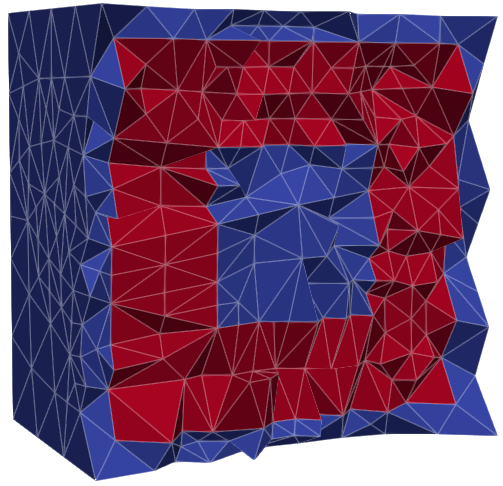
\includegraphics[scale =.14]{ball-2-norm-coarse-mesh-unfitted-3D.png}}; 
   %\draw[] (axis cs:1.75e4,9e-2)   node[right]{{ \resizebox{ 10.5\linewidth}{!}{ \textcolor{black}{$ B \setminus \omega $} } }};
   \draw[] (axis cs:2.5e4,5e-2)   node[draw, fill=white, minimum size=0.5mm]{ \resizebox{ 0.04\linewidth}{!}{ \textcolor{black}{$ B \setminus \omega $}   } };
    %\addplot[orange,very thick,mark=x]  
    %	table[x=ndof,y=rel-L2-err-B] {../data/3d-unfitted-ueval-tuning-p1.dat}; 
    %\legend{ fitted $\mu = (3,30)$,unfitted $\mu = (3,30)$, $\mathcal{O}(h)$   } 	   
    %\legend{ fitted ,unfitted , $\mathcal{O}(h)$   } 	   
        
   
    \nextgroupplot[ 
    ymode=log,
    xmode=log,
    %xmin=0,xmax=1.6e4,
    %xtick={25, 125, 250, 500, 800, 1000},
    %axis x line*=middle,
    %axis y line=middle, 
    xmin = 4e3,
    xmax = 4e6,
    ymin = 3e-2,
    ymax = 2,
    %width=9cm,
    %restrict y to domain=-4e2:4e2,
    %xtick={0,2e3,4e3,6e3,8e3,10e3,12e3,14e3},
    %ytick = {1,0.75,0.5,0.25},  
    xlabel= {ndof},
    %legend pos = south west,
    %legend pos = north east,
    %legend style = { column sep = 2pt, legend columns = 1, at={ (1.0,0.8)},anchor=east},
    %x label style={at={(axis description cs:0.575,-0.15)},anchor=east},
    x label style={at={(axis description cs:0.65,0.075)},anchor=east},
    title = { $p=2$ }, 
    %y tick label style={xshift={3em}}
	]
    
    \addplot[red,very thick,mark=*,forget plot] 
   	table[x=ndof,y=rel-L2-err-B] {../data/3D-comp-fitted-stab-ip-p2-q2-mus(3,30)-ks(10,30).dat}; 
    \addplot[blue,very thick,mark=triangle,forget plot]  
	table[x=ndof,y=rel-L2-err-B] {../data/3D-comp-unfitted-stab--p2-q2-mus(3,30)-ks(10,30).dat}; 
    \addplot[red,very thick,dashed,mark=x,forget plot] 
   	table[x=ndof,y=rel-L2-err-B] {../data/3D-comp-fitted-stab-ip-p2-q2-mus(3,3)-ks(10,30).dat}; 
    \addplot[blue,very thick,dashed,mark=diamond,forget plot]  
	table[x=ndof,y=rel-L2-err-B] {../data/3D-comp-unfitted-stab--p2-q2-mus(3,3)-ks(10,30).dat}; 
    \addplot[gray,dashed,thick,forget plot] 
   	table[mark=none,x=ndof,y expr ={32*\thisrowno{1}}] {../data/3D-comp-unfitted-stab--p2-q2-mus(3,30)-ks(10,30).dat};   %  
    \addplot[gray,densely dotted,thick,forget plot] 
   	table[mark=none,x=ndof,y expr ={700*\thisrowno{1}*\thisrowno{1}}] {../data/3D-comp-unfitted-stab--p2-q2-mus(3,30)-ks(10,30).dat};   %  
     
    \node (meshf) at (axis cs:2.75e4,9e-2) {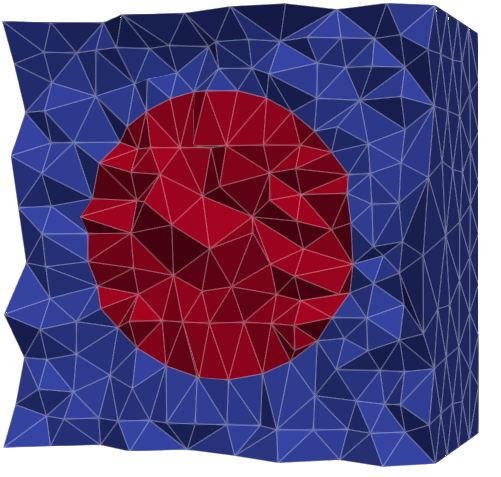
\includegraphics[scale =.14]{ball-2-norm-coarse-mesh-fitted-3D.png}}; 
    \draw[] (axis cs:2.5e4,9e-2)   node[draw, fill=white, minimum size=0.5mm]{ \resizebox{ 0.04\linewidth}{!}{ \textcolor{black}{$ \Omega_1 $}   } };
    %\legend{ fitted $\mu = (3,3)$,unfitted $\mu = (3,3)$, $\mathcal{O}(h^2)$   } 	    
    %\legend{ fitted ,unfitted, $\mathcal{O}(h^2)$   } 	    
        
    \end{groupplot}
    
    \node at ($(group c1r1) + (3.5cm,-3.25cm)$) {\ref{grouplegend}};
    %\node at (0.0,-15.0) {\ref{grouplegend}};
   \end{scope}

  \begin{scope}[yshift=-4.25cm]
  
  \begin{groupplot}[
    group style={
        %group name=rates,
        group size=2 by 2,
        %xticklabels at=edge bottom,
        horizontal sep=30pt,
        vertical sep=5pt,
   },
   %name = dtnplot,
   height = 4.0cm,
   width = 8.0cm,
   every axis plot/.append style={thick},
   %axis y line*=left,
   x label style={at={(axis description cs:0.35,0.085)},anchor=east},
   label style={at={(axis description cs:0.15,0.175)},anchor=north},
   xmin = 0,
   xmax = 1.497,
   ]
   
   \nextgroupplot[ 
	%title = { $p=1$ },
	xlabel= { $x$},
	label style={at={(axis description cs:0.15,0.175)},anchor=north},
	xticklabel=\empty,
        legend pos = north east,
	ymax = 11.5,
	ymin = -3.5,
    ]
    \addplot[lightgray,line width=2pt]
      table[mark=none,x=linecord,y=uval] {../data/3D-comp-fitted-stab-u-eval-reflvl3-p1-mus(3,30)-ks(10,30).dat};
     \addplot[red,solid,line width=1pt,forget plot] 
	    table[mark=none,x=linecord,y=uhval] {../data/3D-comp-fitted-stab-u-eval-reflvl3-p1-mus(3,30)-ks(10,30).dat}; 
     \addplot[blue,solid,line width=1pt,forget plot] 
	    table[mark=none,x=linecord,y=uhval] {../data/3D-comp-unfitted-stab-u-eval-reflvl3-p1-mus(3,30)-ks(10,30).dat}; 	   
	   %\legend{  $u(x,y=0,z=0)$   } 	   
      \addplot[mark=none,dashed,green!70!black,ultra thick ] coordinates {(1.0, -4) (1.0, 12)};
      \node[draw] (CCC1) at (axis cs:0.90,6.5) { $ \Gamma$ };
	  \legend{  $u$   } 	   
   
   \nextgroupplot[ 
	%title = { $p=1$ },
	xlabel= { $x$},
	%label style={at={(axis description cs:0.85,0.175)},anchor=north},
	xticklabel=\empty,
	ymax = 11.5,
	ymin = -3.5,
	%xmin = 0.0,
    ]
    \addplot[lightgray,line width=2pt]
      table[mark=none,x=linecord,y=uval] {../data/3D-comp-fitted-stab-u-eval-reflvl2-p2-mus(3,30)-ks(10,30).dat};
     \addplot[red,solid,line width=1pt] 
	    table[mark=none,x=linecord,y=uhval] {../data/3D-comp-fitted-stab-u-eval-reflvl2-p2-mus(3,30)-ks(10,30).dat}; 
     \addplot[blue,solid,line width=1pt] 
	    table[mark=none,x=linecord,y=uhval] {../data/3D-comp-unfitted-stab-u-eval-reflvl2-p2-mus(3,30)-ks(10,30).dat};
     
    \addplot[mark=none,dashed,yellow!80!black,ultra thick ] coordinates {(0.6, -4) (0.6, 12)};
    
    \node[] (Z1) at (axis cs:0.2,6.5) {};
    \node[] (Z2) at (axis cs:0.05,6.5) {};
    \draw[yellow!80!black,ultra thick,dashed,->] (Z1.east) -- (Z2.west);

    \node[draw] (C1) at (axis cs:0.3,6.5) { $ \omega$ };

    \node[] (K1) at (axis cs:0.4,6.5) {};
    \node[] (K2) at (axis cs:0.55,6.5) {};
    \draw[yellow!80!black,ultra thick,dashed,->] (K1.west) -- (K2.east);


    \node[] (Y2) at (axis cs:0.65,6.5) {};
    \node[] (Y1) at (axis cs:0.825,6.5) {};
    \draw[magenta,ultra thick,dashed,->] (Y1.east) -- (Y2.west);

    \node[draw] (CC1) at (axis cs:1.0,6.5) { $ B \setminus \omega$ };

    \node[] (M1) at (axis cs:1.175,6.5) {};
    \node[] (M2) at (axis cs:1.25,6.5) {};
    \draw[magenta,ultra thick,dashed,->] (M1.west) -- (M2.east);


    \addplot[mark=none,dashed,magenta,ultra thick ] coordinates {(1.3, -4) (1.3, 12)};

   \nextgroupplot[ 
	%title = { $p=1$ },
	xlabel= { $x$},
	%label style={at={(axis description cs:0.85,0.175)},anchor=north},
    ]
    \addplot[lightgray,line width=2pt]
      table[mark=none,x=linecord,y=uval] {../data/3D-comp-fitted-stab-u-eval-reflvl3-p1-mus(3,3)-ks(10,30).dat};
     \addplot[red,dashed,line width=1pt] 
	    table[mark=none,x=linecord,y=uhval] {../data/3D-comp-fitted-stab-u-eval-reflvl3-p1-mus(3,3)-ks(10,30).dat}; 
     \addplot[blue,dashed,line width=1pt] 
	    table[mark=none,x=linecord,y=uhval] {../data/3D-comp-unfitted-stab-u-eval-reflvl3-p1-mus(3,3)-ks(10,30).dat};
   
   \nextgroupplot[ 
	%title = { $p=1$ },
	xlabel= { $x$},
	%label style={at={(axis description cs:0.85,0.175)},anchor=north},
    ]
    \addplot[lightgray,line width=2pt]
      table[mark=none,x=linecord,y=uval] {../data/3D-comp-fitted-stab-u-eval-reflvl2-p2-mus(3,3)-ks(10,30).dat};
     \addplot[red,dashed,line width=1pt] 
	    table[mark=none,x=linecord,y=uhval] {../data/3D-comp-fitted-stab-u-eval-reflvl2-p2-mus(3,3)-ks(10,30).dat}; 
     \addplot[blue,dashed,line width=1pt] 
	    table[mark=none,x=linecord,y=uhval] {../data/3D-comp-unfitted-stab-u-eval-reflvl2-p2-mus(3,3)-ks(10,30).dat};
    \end{groupplot}
  \end{scope}
\end{tikzpicture}
\end{document}





